\documentclass[11pt]{article}
\usepackage{graphicx}
\usepackage{lipsum}
\usepackage{verbatim}
\usepackage{listings}
\usepackage{rotating}
\usepackage[titletoc]{appendix}
\usepackage[left=2.5cm,top=3cm,right=2.5cm,bottom=3cm,bindingoffset=0.5cm]{geometry}
\title{\Huge \textbf{CPU Control} \\ \normalsize \it{Memory Interface and CPU Control \\ Fetch + Decode + Control + Datapath integration}} 
\author{Phillip Bradbury, Zach Toolson, Dan Willoughby}

\begin{document}
\maketitle
\clearpage

\tableofcontents
\clearpage

\section{Overview}
The combination of different modules makes the CPU able to decode assembly instructions, store data in memory, and perform operations. The decoder and controller deal with the parsing of instructions and setting the correct control signals. Dual port memory allows for the memory to be read and written to at the same time. The program counter and instruction FSM work together so that the CPU can execute the various instructions loaded into memory. The layout of the CPU can be seen in Figure \ref{fig:schematic}. The red lines show the control signals, while the black show the flow of the data. Each component, described in detail below, plays an important part in the overall operation of the CPU. 
\begin{center}
\begin{figure}
\caption{Schematic of CPU}
\makebox[\textwidth]{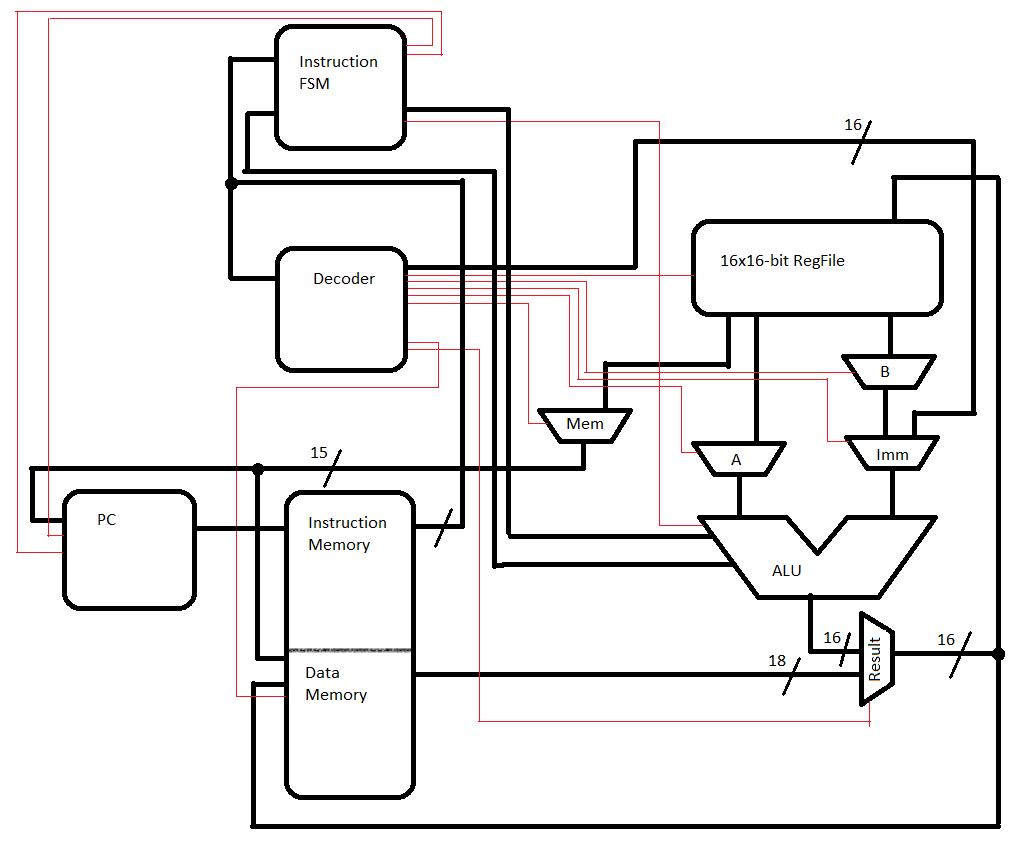
\includegraphics[width=\paperwidth]{cpu.png}}
\label{fig:schematic}
\end{figure} 
\end{center}
\section{ALU}
\subsection{Design}
The ALU designed performs 16-bit integer operations on two inputs. Our ALU performs both addition, subtraction, comparison, logical, and shifting operations on unsigned and signed integers. We treat signed integers using the two’s complement numbers. Most of the design decision came when determining which specific operations we wanted to implement as well as defining what those operations will do. Table 1 shows a list of operations that our ALU implements, as well as each flag that is could possibly throw. Another design decision that we made was to include a carry bit as an input. This was done to make our carry addition and subtraction operations with a carry bit simpler. The inputs and outputs to the ALU are:
\begin{itemize}
\item Input: 1-bit carry 
\item Input: Two 16-bit integers
\item Input: 8-bit opcode
\item Output: 16-bit integer
\item Output: Five 1-bit outputs for each flag described
\end{itemize}
We designed our ALU to follow the CR-16A instructions and opcodes, and only differed in a few cases. The CR-16A specified the behavior of most instructions and what procedure to follow.  One of the differences that we dealt with was implementing the ADDCUI and CMPUI. Since the CR-16A did not have these instructions, we decided to replace the CR-16A SUBCI instruction with ADDCUI and the MULI. Our thought was that the SUBCII and MULI would not be used in our ALU design, so replacing them with alternate instructions would not cause any issues. 

Another difference our ALU had from the CR-16A was the implementation and meaning of flags. The CR-16A specification for flags did not meet our design as closely as we had hoped, and in some cases it was vague. We decided to have a specific meaning for each of the flags, to communicate to the CPU. The meaning of flags we decided on were:
C – The carry bit determines whether a carry occurred after addition or subtraction. 0 means no carry occurred and 1 means that a carry occurred.
L – The low bit is set by the comparison operations. If input A is less than the output Y after the comparison, then the low bit is set to one.
F – The flag bit is used by various operations to signal exceptional situations. This is used show arithmetic overflow in our ALU.
Z – The zero bit is set whenever the output of the operation is zero. This isn’t necessary to set when performing arithmetic operations, but is very useful for comparison operators to signal when the input and output are equal.
N – The negative bit is set by the comparison operators and is set to 1 if the input A is less than the output Y when both are considered to be signed numbers.

\subsection{Implementation}
To implement our ALU design in verilog, we used combinational logic and blocking assignments in the module. We used a case statement in an always block since we knew each op-code. The combinational logic made it easy for us to determine which opcode was given and to perform the corresponding operation. Most of the time we did not need to worry about flags for  an unsigned numbers, so it was simply a verilog operation (E.g. a + b for ADDU). The signed operations required more logic. For the addition operation, we determined the appropriate carry flag with concatenation and performed a check for overflow. Overflow occurred when the inputs most significant bits (MSB) were equal, but the output’s MSB differed. Subtraction also used concatenation for the carry flag, but we needed to check more specific cases for overflow, such as if the inputs had the same sign, but the output did not have the same sign and the result was non-zero.

The remaining operations in our ALU were implemented mostly with verilog operations. We used the verilog shift ( >>, <<) for our shift operations, except the arithmetic shift we made sure that we preserved the sign bit. We were unsure at first how to implement the shift operators because the CR-16A design only had a left shift  (LSH) and arithmetic shift (ASH). We were a bit surprised at the absence of the right shift (RSH), but found out that the CR-16A used negative numbers to have RSH result.  We studied how the CR-16A implemented the shift operations, and then adjusted them to fit our needs. The main difference was that we decided to have a RSH in addition to the LSH instruction. We also expanded on the CR-16A design of the ASH, by adding a ALSH and ARSH ( left and right). We separated the arithmetic instruction so that we could have a simpler approach and ensure the instructions did the correct thing. 

The gate operations AND, OR, XOR, NOT were implemented with the verilog operators \&, |, \^ , ~, respectively. We used subtraction to perform our comparison operations. The two inputs were ‘a‘ and ‘b’. If ‘a’ was less than ‘b’ we set the L flag for unsigned and the N flag for signed. When ‘a’ and ‘b’ were equal we set the Z flag
\section{Memory}
\subsection{Design}
We designed our memory to meet the needs of our duck hunt game. We wanted two separate 16384x18-bit dual-port RAM blocks to allow us to have 4 ports for reading and writing. The reason why we chose to have two RAM blocks, instead of one RAM block(32 blocks of 1024 was the max of the nexys 3 block ram), was so that we could have audio in one RAM block, and game information in the other.
 
We designed our memory to be a synchronous dual-port block RAM. The dual-port memory was so that our program counter could continually read the assembly instructions of the program from one port, while still reading and writing real-time data for the duck hunt game. We established the convention that the top portion of a memory block was the assembly instructions, while the remaining was left for the game data.

\subsection{Implementation}
Our implementation first had a flawed design, but then we reworked it to get one that met our needs. Our initial implementation included 30 separate blocks of memory. Each block was 1024 registers and we wanted to tie 30 blocks together, leaving two blocks for audio.  The idea behind having 30 blocks and 2 blocks, was so that we could have two ports for the 30 blocks and two ports for the remaining 2 blocks. The initial implementation had issues with the \$readmemh command. Because of the instantiation issue we decided to redesign the memory from scratch.
 
The next implementation of our memory followed closely to the example code given in lab. The code includes two read/write ports, each having its own data in and data out bus. It also had a separate clock for each port. We decided when we instantiated the memory module, to pass in the same clock as an argument. Using the same clock for both memories had no negative effect on the function of the memory. The memory module used two parameters for the data and the address. The parameters were set to a default value in the module. When instantiating the module to use the programmer can then change the variable values if desired. We set two parameters to the values of data = 18, and addr = 14. These numbers are based on the Block-RAM design of the Spartan 6 board, which gave us 32 blocks of RAM, with each block having 18k bits. Xilinx tools requires a special syntax to declare the memory, which we followed using the reg [DATA-1:0] mem [(2**ADDR)-1:0] command. We then use the \$readmemh command to read in a file and instantiate the memory with our game code at compile time. To implement our read/write memory design in Verilog we check if the memory should be writing or reading. When the positive edge of the clock hits, check to see if the memory is set to write. If it is, read the data out first before writing the incoming data, otherwise just read the data out of the address requested. This is a read-first memory design. With this second design, out memory worked properly and met the needs of our game design.

\subsection{RegFile Integration}
    The RegFile contained 16 registers, which was implemented using a combination of non-blocking statements. Each register had a clock, reset, enable, input, and output. To implement a register we used an if/else statement; when the register was enabled the input was set as the output, otherwise the register would display the output. The xilinx tools synthesized our register implementation to a D-Flip-flop, which was the expected behavior. 

    We ran into some issues when we first implemented our RegFile. We created multiple modules in our RegFile, which added to the complexity. Instead of just have 16 registers in the file, we had most of the data path as well. We resolved the issue by separating the modules into separate verilog files. Doing so allowed for a simpler RegFile and ease of debugging. Another issue we encountered was connecting the reset control signal. We first thought that each register needed to be reset independently. As a result, we started adding additional logic to allow for the separate resets. After a while, we concluded that the reset signal should reset all of the registers at once. The signal reset control signal greatly simplified our RegFile design. 

\section{Instruction FSM}
\subsection{Design}
The instruction FSM design was meant to give a life cycle for each assembly instruction. Depending on which instruction was read from memory, it took a longer or shorter amount of time to execute it. For example, a stor/load instruction can take up to 4 clock cycles while a non memory instruction takes only 3 clock cycles. We needed an FSM to account for these differences so that each instruction can work. We designed our FSM to be a moore finite state machine so the output only depended on the current state. The instruction FSM interacted with the PC counter with control signals.

The FSM has three main functions. One function that the FSM did was set the PC counter to an address which was read from a register(branches and jump). Another function was to increment the PC counter(for the next assembly instruction). The last main function was to interact with the ALU flags. Each state in the FSM corresponds to its function described in \ref{table:state}. The next state logic of the FSM ensured that each instruction was allowed enough time to execute fully.

\begin{table}
\centering
\caption{Description of instruction FSM states}
\begin{tabular}{|c|p{4in}|}
\hline
State & Description \\
\hline
fetch & Initial state, sets up the address for Instruction Memory \\
decode & After getting the data-out from the Instruction Memory \\
alu & After decode state, then goes straight to fetch \\
stor1 & State after decode which waits several cycles \\
stor2 & When output recieved, sets up the instructions to push to the register \\
load1 & State after decode which waits several cycles \\
load2 &  When output of memory is recievied signals the data was loaded \\
jump & Sets up the program counter with the new address \\
\hline
\end{tabular}
\label{table:state}
\end{table}

\subsection{Implementation}
The instruction FSM was implemented using a moore finite state machine design. We had present state logic, next state logic, and output logic each with its own associated always block statements. The present state logic had a sensitivity list to execute on the positive edge of the clock. If it was set to clear, then the present state would be set to fetch and the flags would be reloaded. Otherwise, the present state would be set to the next state. We also included some logic to fetch the flags from the ALU which made it so it took two cycles for the flags to actually change. We verified through testing that the flags were being set properly and it had no negative effect with our state machine. 

The next state logic always block determined the next state based off the the present state. For example, if the present state was fetch, the next state would be set to decode. Likewise, if the present state was decode, the next state would be determined by the decoded instruction. In this case, if it was a load instruction it would set to the load1 state(see \ref{table:state}). The rest of the next state states were determined in a similar fashion, always with the end result of the next state being set to the fetch state. 

The output logic block set the control signals to the ALU and the PC counter. For certain instructions such as branch, the FSM checked the flags set by the ALU. If it was a BEQ instruction, the FSM would determine if the zero flag was high and set the appropriate control signals. We also included some logic for compare operations, so that the flags had ample time to be set.
 

Another main issue we encountered was that was that we did not have enough states for our instructions. This was a problem because the compare operation required a different amount of time than a simple ALU instruction. As a result, the problem encountered was that the branch instructions were not working correctly. For example, a BEQ would always branch instead of only branching when they are equal (zero flag =1 ). We resolved the problem by creating additional states for the compare instructions. The additional states allowed for the flags to be set and read correctly for the branch or jump instructions. 

Another main issue we encountered was with the load and store instructions not reading or loading the correct register. The incorrect register caused the output of the ALU to be undetermined (XXX). The undetermined output was an issue because we could not communicate with the reg file the appropriate value or address to be extracted from memory. We discovered that our datapath from memory that connected to the ALU-out datapath needed to have additional logic (needed a mux). The additional logic ensured that we were setting the memory data-out to the ALU-out datapath at the correct time. After we overcame these issues, the instruction FSM functioned properly.

\section{Decoder}

\subsection{Design}
The purpose of our decoder was to abstract away the decoding of the assembly instructions and send control signals to other components of the CPU. We had it separate from the instruction FSM so that it was easier to debug. Each instruction was parsed by 4 bit chunks. It would read the opcode,  opcode extension, the register destination / source / address, and immediate value. We had the decoder deal with reading 2’s complement immediate values. For example, if the instruction was addi we would extend the most significant bit sign to fill up the remaining 16 bits. 

After the assembly instruction was parsed, it would set the control signals corresponding to the instruction’s opcode. The decoder was responsible for communicating with the reg file, the memory, and muxes that control the flow of the datapath. 

\subsection{Implementation}
The implementation of the decoder required using a case statement to set each control signal. The register control signals needed to communicate to the reg file when to write and which register to read or write to or from, respectively. The first case statement was on the top 4 bits of the instruction (15:12). These 4 bits determine if the instruction was a register type instruction (add \$1, \$2), or any other instruction (immediate, shift, compare, branch, etc). We then had another case statement of the opcode extension bits (7:4) and it would set the opcode to communicate to the ALU which registers to read and load to the reg file.

The immediate instructions were similar to the register type instruction, except it would load in an immediate value. We had a case for each instruction that dealt with immediate values. The decoder would read in the immediate value from the instruction, extend the MSB if it was 2’s complement, and enabled the mux that allowed for an external immediate value to be loaded into the ALU. The immediate value would come from the decoder and be sent to the B port of the ALU. The compare and move immediate instructions were done in a similar fashion. The shift instructions required no extra logic to decode and worked similar to the register type instruction that they correlated with.

The last case was when we had a memory or branch type instruction. We decided to have the branch, jump, load, and store instructions have the same opcode. The reason was because we did not think that we would have very many branch instructions. The way the decoder differentiated between the branch instructions and the actual memory instructions (load / store) was by the opcode extension. The load instruction was responsible for enabling a control signal that switched the ALU-out bus to the B data-out port of the memory. This allowed for the value stored in memory to be loaded directly into the datapath. The store instruction was responsible for setting the write enable signal to the memory module. Both the load and store instructions set the B port address to be read/loaded. The decoder’s job with the branch and load instruction was to tell the reg file which registers to read and load to. The 4 LSB (3:0) specified which type of condition the branch was (equal, not equal, jump). The instruction FSM dealt with reading the flags of the ALU and which address to jump to. With the case statement on each instruction, it allowed us to easily implement the decoder.



\section{Program Counter}
\subsection{Design}
The goal for our program counter was simplicity. We moved some of the complicated things into our assembly code design and dealt with the problems there. This includes signed 2’s complement addresses and signed offsets. The program counter was designed so that we could set it to any address. We also allowed for the PC counter to be incremented by any value. The conventions we established were that addresses used to set the program counter must be an unsigned number. By setting some conventions, we greatly simplified our program counter.

\subsection{Implementation}
The program counter would increase each clock cycle by the increment value provided. The instruction FSM communicated to the PC counter how much to increment by. The main purpose behind having the increment being externally controlled was so that the instruction FSM could tell the PC counter when to increment. For example, when we did not want the program counter to increment, we would set the increment value to zero. When we did want it to increment, we would set the value to one. The external increment value also allowed us to have a jump instruction which would set the increment value to however far we wanted the program counter to jump. The increment value could be positive or negative. We used an always block with the posedge of the clock in the sensitivity list. The program counter would increment the output address by the increment value given unless an address was being set. In this case, the output address would become the input address. The instruction FSM was responsible for all of the life cycle of instructions. Therefore, we could have a relatively simple program counter.


\section{CPU Datapath}
\subsection{Design}
The CPU datapath’s purpose was to instantiate all the modules, and to connect them all together. We instantiated each module, and then created wires to connect the inputs and outputs of the modules to each other. For example, we needed to connect the memory to the instruction FSM, decoder, and ALU. We abstracted the decoder and instruction FSM into its own module called the controller. The controller instantiated the required muxes / wires to communicate effectively between the decoder and instruction FSM.  The program counter needed to be connected to the controller and the memory. Because we abstracted most of the details away into separate modules, the CPU datapath was relatively straightforward. 

\subsection{Implementation}
The implementation of our CPU was instantiating modules and connecting them together. We instantiated the program counter, memory, and controller and then tied their inputs and outputs to their designated places. For documentation purposes, we declared each wire that connected the modules. We also had several outputs of different signals to aide us with debugging. The final addition to out CPU was a clock divider to allow enough time for instructions to be executed on the board. With all the modules connected, the CPU was able to execute a simple program.




\section{ Waveforms of test operation }
\subsection{Phase i}
Loads data from memory into RegFile. Refer to Figure. \ref{fig:p1}. 

\subsection{Phase ii}
Performs a series of arithmetic and logical operations. Refer to Figure. \ref{fig:p2}. 

\subsection{Phase iii and Phase iv}
Stores the result into memory and reloads the result from memory into the RegFile.  Refer to Figure. \ref{fig:p3}. 

\subsection{Phase v and Phase vi}
Performs arithmetic to set flags and uses flags to perform branches. We implemented a loop that calls a method that displays the numbers 1 to 5, each iteration. Refer to Figure. \ref{fig:p4}. 

\subsection{Phase vii}
Writes the result into memory and displays the result. Refer to Figure. \ref{fig:p5}. 


\section{Conclusion}
The results of Lab 3 and Lab 4 were that we were able to run our own assembly programs on our CPU. We found several errors as we were testing, which we were able to correct. It would have been near impossible to test the CPU without the different components seperated into different modules. The combination of all the modules formed a complex design, which could perform interesting operations. The CPU successfully running a program we wrote was very exciting and encouraging. 


\newpage
\appendixname
\appendix
\section{Synthesis Results}
\subsection{Memory}

\end{document}
